%   Filename    : chapter_4.tex 

\chapter{Preliminary Results}
This chapter outlines the results of preprocessing, training of machine learning models, and feature importance analysis. The dataset was preprocessed using Python in Google Colab. After preprocessing, the dataset was imported to MATLAB to train and evaluate the performance of various classifiers. It was followed by assessing the performance of different classifiers and conducting feature importance analysis to identify the most significant predictors for sex identification in \textit{T. granosa}.

\section{Data Summary}
\subsection{Dataset Overview and Exploration}

The dataset contains the morphometric measurements collected from the 77 male and 72 female T. granosa samples. Figure no. shows the proportion of male and female samples, a total of 149 samples collected by the researchers and classified through spawning and dissection. 

\newpage

\begin{figure}[!htbp]
	\centering
	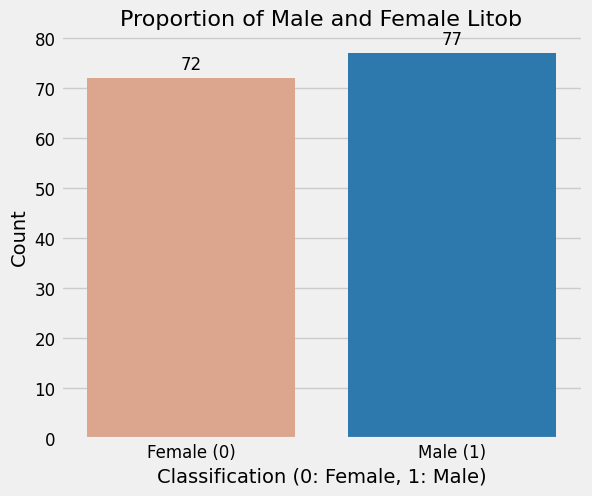
\includegraphics[width=0.8\textwidth]{figures/test-train.png}
	\caption{Proportion of Male and Female \Tgranosa}
	\label{fig:test-train}
\end{figure}

\begin{figure}[!htbp]
	\centering
	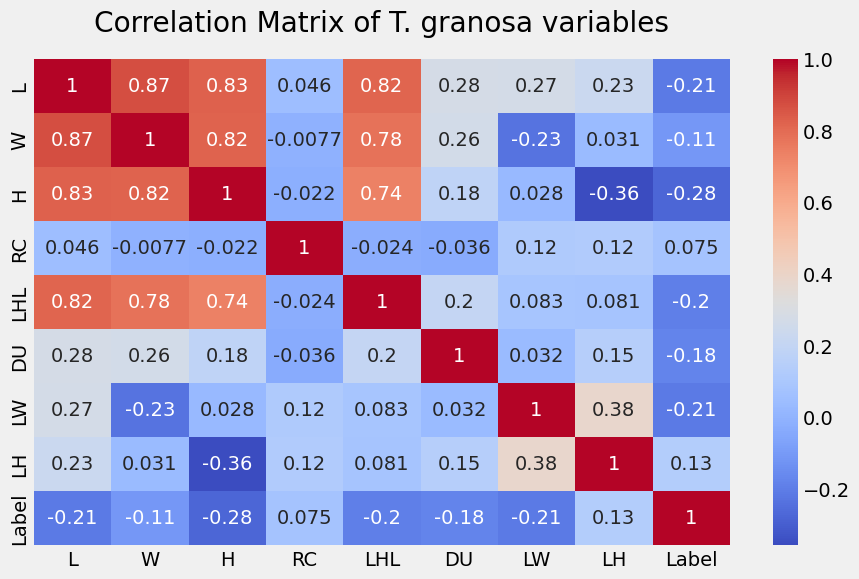
\includegraphics[width=0.8\textwidth]{figures/corr_matrix.png}
	\caption{Correlation Matrix of Predictors and Target Variables}
	\label{fig:corr-matrix}
\end{figure}
\newpage
Figure~\ref{fig:corr-matrix} shows the correlation matrix between the variables and the correlation with the target was identified and displayed in the heatmap. The positive correlations observed in the matrix are the length (L) and Width (W) having (r = 0.87) and height (H) (r = 0.83), width (W) and Height (H) with (r = 0.82), and length (L) and hinge line length (LHL) with (r = 0.82). These features show high multicollinearity since the correlation is greater than 0.8 \cite{kim2019}. This feature indicates that as the length of the shell increases, its width, height, and hinge line length increases as well. In contrast, the rib count (RC) and distance of the umbos (DU) have a weak correlation from other features, with (r = 0.0046) and (r = 0.28) being the highest, respectively. This indicates that features such as the rib count and distance of the umbos do not strongly depend on the length, width, and height of the shell. 
The correlation analysis between the predictors and the target (label, male or female) showed that most features had a weak negative correlation with the label. Specifically, the highest negative correlations were observed for the length (L) (r = -0.21),  and height (H) (r = -0.28) being the highest, indicating that these linear measurements only slightly differ between males and females, making it challenging to distinguish morphometric differences. Conversely, a weak positive correlation was found between the label and the rib count (RC) and the length-to-height ratio (LH\_ratio), implying that as these variables increase, the likelihood of classifying the sex improves.

Overall, the results show that while linear measurements such as length (L), width (W), height (H), and hinge line length (LHL) are interdependent, the rib count (RC) and distance between umbos (DU) are mostly independent features. Additionally, the weak correlations between the linear measurements and the label suggest that distinguishing between male and female \Tgranosa based on these traits alone is difficult. To enhance predictive power, a combination of features should be considered. Feature selection could be employed to identify meaningful combinations of features and evaluate their performance using machine learning metrics. Identifying these patterns is crucial for understanding complex biological processes, as traditional correlation coefficients that capture only linear relationships may overlook nonlinear interactions \cite{pividori2024}.


\subsection{Statistical Analysis of \Tgranosa features}

\begin{table}[H]
	\centering
	{\fontsize{8}{10}\selectfont 
		\resizebox{\linewidth}{!}{ 
			\begin{tabular}{lcccc}
				\hline
				\textbf{Feature} & \textbf{$Mean \pm SD$} & \textbf{Min} & \textbf{Max} & \textbf{p-value}  \\ \hline
				Length              & $46.41 \pm 5.01$ & 38.050000 & 64.800000 & 0.036142  \\
				Width               & $35.66 \pm 3.78$ & 28.250000 & 45.500000 & 0.255091  \\
				Height              & $32.10 \pm 3.59$ & 23.350000 & 45.050000 & 0.000577  \\
				Rib count           & $19.65 \pm 0.88$ & 17.000000 & 22.000000 & 0.333161  \\
				Length (Hinge Line) & $28.06 \pm 4.24$ & 20.050000 & 43.050000 & 0.020658  \\
				Distance Umbos      & $3.25 \pm 2.85$ & 1.050000 & 35.050000 & 0.000874  \\
				LW\_ratio            & $1.30 \pm 0.07$ & 1.114710 & 1.692185 & 0.026395  \\
				LH\_ratio            & $1.45 \pm 0.10$ & 1.191919 & 1.844398 & 0.086674  \\
				\hline
			\end{tabular}
		}
	}
	\caption{ Dataset Overview and Exploration}
	\label{tab:descriptive-stat}
\end{table}

Table~\ref{tab:descriptive-stat} shows a statistical summary of the different features, including the mean, standard deviation, minimum, maximum, and p-values, indicating the distribution across the sampled population. These values provide insight into the characteristics and sizes of \textit{T. granosa}. 

Standard deviation measures the variation in a set of data values around their respective mean. Among the eight features, the distance between the umbos shows the highest variability (SD = 2.85), indicating that this feature varies significantly among samples. In contrast, rib count demonstrated the lowest variability (SD = 0.88), suggesting that this feature is relatively consistent across the dataset. Other features displayed moderate standard deviation values, indicating low to moderate variability.

A normality test was performed to determine the distribution of the samples. The results revealed that all samples followed a non-normal distribution. Subsequently, the Mann-Whitney U test was carried out to calculate the p-values. Out of the eight features, five were found to be statistically significant: Length (p-value = 0.036142), Height (p-value = 0.000577), Hinge Line Length (p-value = 0.020658), Distance Between Umbos (p-value = 0.000874), and LW\_ratio (p-value = 0.026395). With a 95\% confidence interval, these features were statistically significant in relation to the target Label. These results suggest that these five features are important predictors influencing sex determination. Further analysis such as feature importance would be conducted to validate and quantify their contribution.  


\section{Comparison of Model Performance}
\begin{figure}[!htbp]
	\centering
	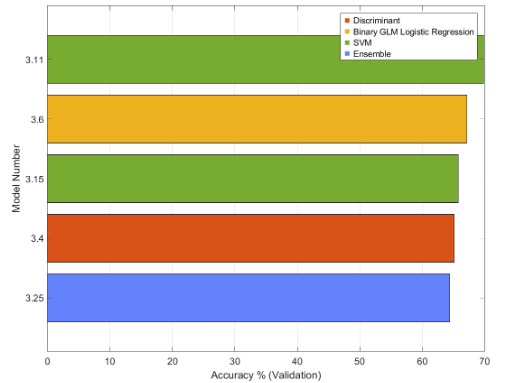
\includegraphics[width=0.6\textwidth]{figures/compare-models.png}
	\caption{Comparison of Model Performance}
	\label{fig:compare-models}
\end{figure}

Figure~\ref{fig:compare-models} shows the comparison of the accuracy in classifying the sex of T.granosa across different models including Discriminant, Binary GLM Logistic Regression, SVM, and Ensemble. Based on the figure above, the SVM achieved the highest accuracy percentage of 69.80\%. This indicates that the SVM performed best among the models in the validation set, followed by the Binary GLM Logistic Regression and then the Discriminant. On the other hand, the Ensemble had the lowest accuracy making it the least effective model in the validation set. 

\subsection{Performance Evaluation}

To evaluate the performance of the different models used, the effectiveness of each model in predicting the sex of \Tgranosa based on morphometric characteristics was assessed and compared. Performance metrics such as accuracy, precision, recall, and F1-score were utilized to evaluate the models. By analyzing these metrics, the researchers can identify the most effective model for classifying male and female \textit{T. granosa}.


\begin{table}[H]
	\centering
	\resizebox{\linewidth}{!}{ 
		\begin{tabular}{lccccc}
			\hline
			\textbf{Model} & \textbf{Accuracy (Validation)} & \textbf{ Weighted Precision} & \textbf{ Weighted Recall} & \textbf{Weighted F1-score} & \textbf{Training Time (sec)} \\ \hline
			Linear SVM          & 69.80(\%) & 69.82(\%) & 69.80(\%) & 69.73(\%) & 2.354 \\
			Binary GLM Logistic Regression    & 67.11 (\%) & 67.16(\%) & 67.11(\%) & 66.99(\%) & 1.9415 \\
			Medium Gaussian SVM       & 65.77(\%) & 65.77(\%) & 65.77(\%) & 65.69 (\%) & 1.0323 \\
			Linear Discriminant       & 65.10(\%) & 65.22(\%) & 65.10(\%) & 64.86(\%) & 2.333\\
			Subspace Discriminant     & 64.43(\%) & 64.50(\%) & 64.43(\%) & 64.23(\%) & 7.708 \\ \hline
		\end{tabular}
	}
	\caption{Performance Metrics of Machine Learning Models for Sex Identification}
	\label{tab:model-performance}
\end{table}

Table ~\ref{tab:model-performance} presents the comparison results of machine learning models on the morphometric characteristics of the combined- male and female \textit{T.granosa} datasets. The results indicate that all models demonstrated moderate to high performance in predicting males and females, with accuracies ranging between 64.43\% to 69.80\%. 

The Linear SVM performs as the best model achieving the highest accuracy (69.80\%), precision (69.82\%), recall (69.80\%), and F1-score (69.73\%), with a training time of 2.354s. This indicates that SVM is well-suited in identifying sex of \textit{T.granosa} based on its morphological features. 

The Binary GLM Logistic Regression also performed well having an accuracy of 67.11\%, precision of 67.16\%, recall of 67.11\%, and F1-score of 66.99\%, with a training time of 1.9415s which is faster than Linear SVM. 

The Medium Gaussian SVM, and Linear Discriminant closely followed each other with accuracies of 65.77\% and 65.10\%, precisions of 65.77\% and 65.22\%, recalls of 65.77\% and 65.10\%, and F1-scores of 65.69\% and 64.86\%, with a training time of 1.0323s and 2.333s, respectively. 

The Subspace discriminant, however, performed as the worst classifier with an accuracy of 64.43\%, precision (64.50\%), recall(64.43\%), and F1-score (64.23\%), having the longest training time of 7.708s. 

Overall, the results seen in this comparison highlight that machine learning models are effective in predicting sex identification of \textit{T.granosa} based on their morphometric characteristic with Linear SVM performing as the best model for this dataset. 


\subsection{Confusion Matrix Analysis}
\begin{figure}[!htbp]
	\centering
	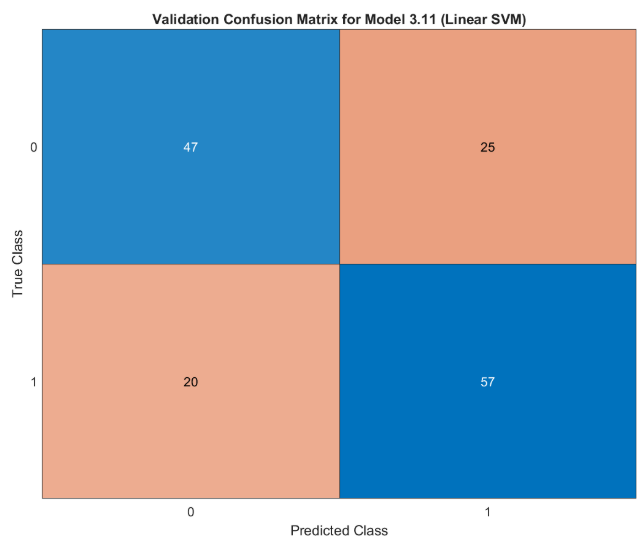
\includegraphics[width=0.6\textwidth]{figures/confusion-matrix.png}
	\caption{Confusion Matrix of Linear SVM}
	\label{fig:confusion-matrix}
\end{figure}

Figure~\ref{fig:confusion-matrix} displays the confusion matrix that provides a detailed breakdown of classifier predictions, including true positives (correctly identified females), true negatives (correctly identified males), false positives (males incorrectly classified as females), and false negatives (females incorrectly classified as males).

The Linear SVM, being the best performing model, achieved 57 true positives and 47 true negatives. However, it also had 25 false positives and 20 false negatives. This indicates that the model did not accurately differentiate between male and female, aligning with its accuracy of 69.80\%. The large number of incorrectly classified data points suggests while the Linear SVM is the best model compared to others, it still struggles with the complexity of this dataset. 

\newpage
\subsection{Feature Importance Analysis}

\begin{figure}[!htbp]
	\centering
	\begin{minipage}{0.48\textwidth} 
		\centering
		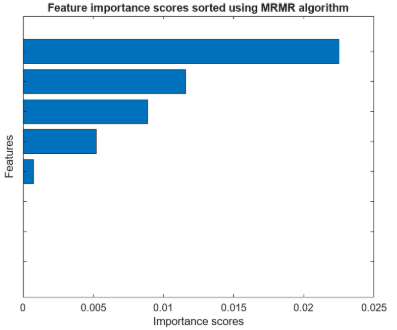
\includegraphics[width=\textwidth, height=5cm]{figures/mrmr.png} 
	\end{minipage}%
	\hfill 
	\begin{minipage}{0.48\textwidth} 
		\centering
		{\fontsize{12}{15}\selectfont 
			\begin{tabular}{p{0.5\linewidth}c}
				\hline
				\textbf{Features} & \textbf{MRMR Scores} \\ \hline
				Height              & 0.0225  \\
				Lw\_ratio           & 0.0116  \\
				DistanceUmbos       & 0.0089  \\
				RibCount            & 0.0052  \\
				Length              & 0.0007  \\
				\hline
			\end{tabular}
		}
	\end{minipage}
	\caption{Feature Importance Scores Sorted Using the MRMR Algorithm.}
	\label{fig:mrmr-combined}
\end{figure}

\begin{figure}[!htbp]
	\centering
	\begin{minipage}{0.48\textwidth} 
		\centering
		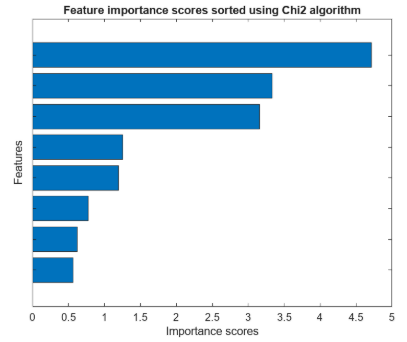
\includegraphics[width=\textwidth, height=5cm]{figures/chi2.png} 
	\end{minipage}%
	\hfill 
	\begin{minipage}{0.48\textwidth} 
		\centering
		{\fontsize{12}{15}\selectfont 
			\begin{tabular}{p{0.5\linewidth}c}
				\hline
				\textbf{Features} & \textbf{Chi2 Scores}   \\ \hline
				DistanceUmbos       & 4.7164   \\
				Height              & 3.3334  \\
				Length\_Hinge\_Line & 3.1542  \\
				LW\_ratio           & 1.2570  \\
				Length              & 1.1934  \\
				RibCount            & 0.7718 \\
				LH\_ratio           & 0.6241 \\ 
				Width               & 0.5611 \\ 
				\hline
			\end{tabular}
		}
	\end{minipage}
	\caption{Feature Importance Scores Sorted Using the Chi2 Algorithm.}
	\label{fig:chi2-combined}
\end{figure}

\begin{figure}[!htbp]
	\centering
	\begin{minipage}{0.48\textwidth} 
		\centering
		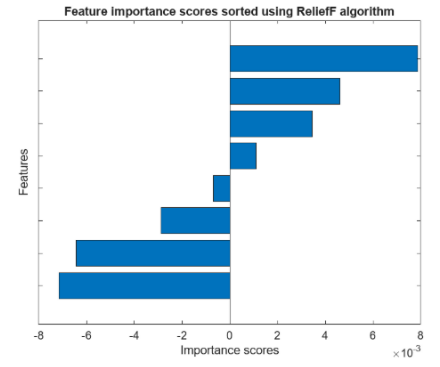
\includegraphics[width=\textwidth, height=5cm]{figures/reliefF.png} 
	\end{minipage}%
	\hfill 
	\begin{minipage}{0.48\textwidth} 
		\centering
		{\fontsize{12}{15}\selectfont 
			\begin{tabular}{p{0.5\linewidth}c}
				\hline
				\textbf{Features} & \textbf{ReliefF Scores}   \\ \hline
				DistanceUmbos       & 0.0079   \\
				Length              & 0.0046  \\
				Width               & 0.0034  \\
				Length\_Hinge\_Line & 0.0011  \\
				\hline
			\end{tabular}
		}
	\end{minipage}
	\caption{Feature Importance Scores Sorted Using the ReliefF Algorithm.}
	\label{fig:reliefF-combined}
\end{figure}

\begin{figure}[!htbp]
	\centering
	\begin{minipage}{0.48\textwidth} 
		\centering
		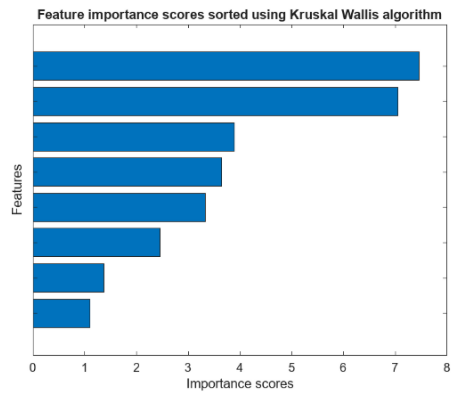
\includegraphics[width=\textwidth, height=5cm]{figures/kw.png} 
	\end{minipage}%
	\hfill 
	\begin{minipage}{0.48\textwidth} 
		\centering
		{\fontsize{10}{12}\selectfont 
			\begin{tabular}{p{0.5\linewidth}c}
				\hline
				\textbf{Features} & \textbf{Kruskal Wallis Scores}   \\ \hline
				Height              & 7.4640  \\
				DistanceUmbos       & 7.0491  \\
				Length\_Hinge\_Line & 3.8847  \\
				LW\_ratio           & 3.6395  \\
				Length              & 3.3250 \\ 
				LH\_ratio           & 2.4496 \\
				Width               & 1.3692 \\
				RibCount            & 1.1022 \\
				\hline
			\end{tabular}
		}
	\end{minipage}
	\caption{Feature Importance Scores Sorted Using the Kruskal Wallis Algorithm.}
	\label{fig:kw-combined}
\end{figure}

\newpage

After processing the dataset and splitting it into training and testing sets, the models are trained and their important features are computed. The features are further reduced in the table removing zeros and negative results that do not contribute to the scores. Feature Analysis helps in identifying which morphological features contribute most in classifying male and female T.granosa. The study employed models such as Minimum Redundancy Maximum Relevance (mRMR), Chi-square (Chi2), ReliefF, Analysis of Variance (ANOVA), and Kruskal Wallis feature selection algorithms. 

The Minimum Redundancy Maximum Relevance (mRMR) identified the best features as height, LW ratio, distance of the umbos, rib count, and length respectively, which contribute most to sex classification. The Chi-square (Chi2) analysis includes all eight features: however, the distance of the umbos is the most significant, followed by height, length of the hinge line, LW ratio, length, rib count, LH ratio, and width. In the ReliefF scores, the key features include the distance of the umbos, length, width, and length of the hinge line, while height, LW ratio, LH ratio, and rib count did not contribute to sex classification. Furthermore, in the Kruskal-Wallis analysis, height is the most significant feature, followed by the distance of the umbos, length of the hinge line, LW ratio, length, LH ratio, width, and rib count as the least significant.

The results in figures~\ref{fig:mrmr-combined},~\ref{fig:chi2-combined},~\ref{fig:reliefF-combined}, and~\ref{fig:kw-combined} indicate variations in feature importance among the four algorithm models. However, certain features, such as the distance between the umbos, are present in the best features of all algorithms, followed closely by height, which is identified as a key feature in three of the four models, except for ReliefF. Therefore, features such as the distance between the umbos and height consistently emerge as influential predictors. This analysis enabled the researchers to identify the most predictive features, which can serve as a baseline for sex identification of T. granosa based on morphological characteristics. 




